\chapter{Design and Implementation}

\section{Introduction}
In this chapter all aspects of design and implementation that were done for this project are discussed. A parallel infrastructure was essential for this project for implementing the PGA using Message Passing Interface. A considerable time and effort were made to implement and configure the Beowulf cluster to facilitate the parallel infrastructure for the project. Our original idea was to use an existing Beowulf system in University's laboratory. Later it was discovered that, the most of the hardware of that Beowulf system were dismounted and no longer suitable for this project. So, the the most obvious alternative was to build a Beowulf cluster for this project. At first, a virtual Beowulf system was simulated on a dual core MacBook. Then an actual hardware based Beowulf system was implemented using multiple old PC's. After all, this is the noble idea of a Beowulf system to have it built using hardware laying around  that have very little or no use at all.

Another important part of implementing a PGA, we needed to identify a suitable existing SGA implementation. Even though the Genetic Algorithm was not the centre theme of this project, it was very important to do a considerable background studies in GA to understand the underlying concepts well. It was also important to understand and identify different techniques of parallelising GAs. Much efforts and time were put into understanding two different implementation of SGA and their suitability on parallelising using MPI in details for this project which are discussed in this chapter.

With PGA implementation, we were faced with many issues and challenges. Some of these issues were identified during PGA implementation and some were identified during empirical studies. Which resulted in implementing 3 versions of PGA. 

A lot efforts were made to create prototypes using python scripts to gather experiments data and use gnuplot to visualise the results to compare and contrast to validate the hypotheses relating to PGA performance.

\section{Setting up the Beowulf Cluster}
\label{beowulf_setup}
\subsection{Cluster components}
Computer cluster is made up of various hardware and software components with complex interactions between different components. Figure \ref{fig:cluster-layers} depicts the various components that form a cluster.

\begin{figure}[!htb]
 \center
  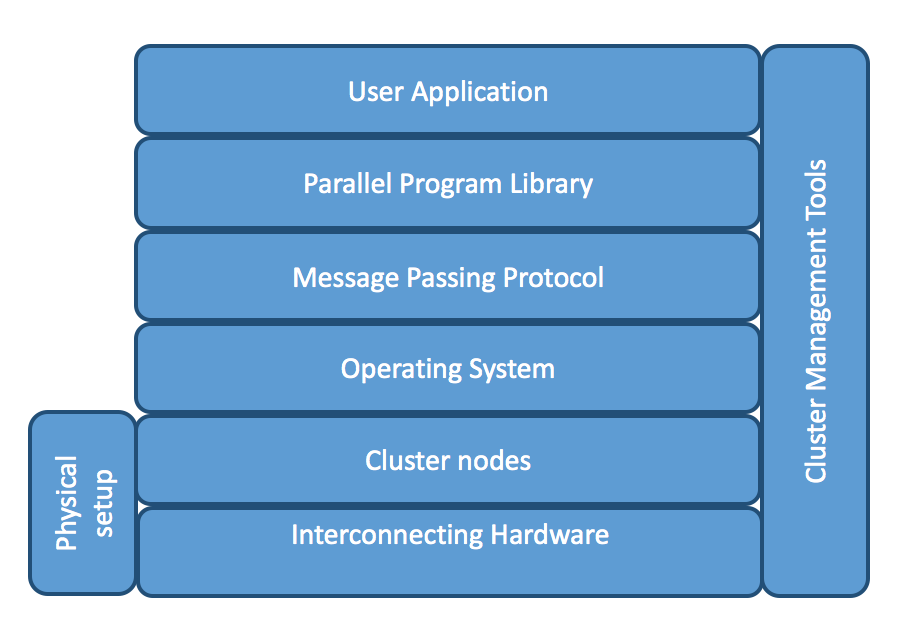
\includegraphics[width= .75 \linewidth]{figs/cluster/cluster_layers.png}
  \caption{Layers in a Cluster}
  \label{fig:cluster-layers}
   \center
\end{figure}

A Beowulf cluster contains a set of cluster nodes. A node can be a server with a specific role within the cluster or it can be a compute node. All of the nodes are connected using a dedicated Local Area Network(LAN) or System Area Network(SAN). The complexity of networking topology is depends on directly to number of nodes in the cluster.

As shown in Figure \ref{fig:cluster-layers} to setup a cluster we need following hardware and software components:

\paragraph{Cluster Nodes}
Cluster nodes are stand-alone computers with one or more CPUs, own Memory unit, and Network Interface Card(NIC). A node may contain it's own local secondary storage or could be configured as disk-less workstation. For this implementation nodes were configured with their own local storage to reduce network overhead for accessing boot-image and runtime libraries during boot up and program execution. However, Network File Sharing(NFS) was implemented to streamline program execution environments across the Cluster. The details of nodes configurations are discussed later in this chapter for both virtual and physical implementation.

\paragraph{Interconnecting Hardware}
This is networking components of the cluster that facilitates nodes communicating with one another. Since communication is the key part of cluster computing this is very important component that can define the overall performance. For this project a simple ethernet network was configured for both virtual and physical implementation. For the physical setup, Thompson Broadband Router (Model: TWG870) was used. This router has 4 Gigabit ports that facilitated to setup a Gigabit LAN for the cluster-only network.

\paragraph{Operating System}
Linux is widely used on Beowulf cluster because of its hardware support, performance, its free and open source kernel. For this project Ubuntu Server 16.04 was chosen.

\paragraph {Message Passing Protocol}
There are two typical approaches to communication between cluster nodes, one is  Parallel Virtual Machine(PVM) and the other is Message Passing Interface (MPI). However, MPI has now emerged as the de facto standard for message passing on computer clusters. The objective of this project is parallelising SGA using MPI libraries therefore, MPI was chosen message passing protocol for obvious reason.

\paragraph {Parallel Program Library}
MPI has many implementation. There are two free and popular MPI libraries available, one is OpenMPI and another is MPICH. For this project MPICH 3.2 is installed on each nodes. 

\paragraph {Cluster management tools}

\subsection{Topological design}
Figure \ref{fig:beowulf-cluster} shows a simple Beowulf cluster setup that was adopted for this project implementation. For simplicity the implemented Beowulf contains a Master node and 3 to 4 compute nodes which is extendable.

\begin{figure}[!htb]
  \includegraphics[width=\linewidth]{figs/cluster/beowulf_cluster.png}
  \caption{A typical Beowulf setup}
  \label{fig:beowulf-cluster}
\end{figure}

Beowulf cluster was simulated in virtual environment using Oracle VirtualBox and then actual hardware implementation was done using commodity physical hardware. In both cases the software suits and configuration was identical with minor changes.

\subsection{Virtual nodes}
Table \ref{tab:virt_node_conf} shows the node configuration when using simulated hardware using VirtualBox on Macbook Pro(2.6GHz Intel core i5, 16 GB RAM, 256GB SSD) host computer.

%% Node description table 
\begin{table}[!htb]
\centering
\caption{Virtual nodes configuration}
\begin{tabular}{|l|l|l|l|}
\hline
Hostname & Role & IPv4 address & Hardware Config \\ \hline
master & Master & 192.168.56.10/24 & Single core, 2GB RAM, 10 GB HDD \\ \hline
node1 & Slave & 192.168.56.11/24 & Single core, 2GB RAM, 10 GB HDD \\ \hline
\end{tabular}
\label{tab:virt_node_conf}
\end{table}

\subsection{Physical nodes}
Table \ref{tab:phy_node_conf} shows the node configuration of using physical components. 
%% Physicle node description table 
\begin{table}[!htb]
\centering
\caption{Physical nodes configuration}
\begin{tabular}{|l|l|l|l|}
\hline
Hostname & Role & IPv4 address & Hardware Config \\ \hline
padma & Master & 172.16.0.1/24 & Dell Dual-core, 6GB RAM, 160 GB HDD \\ \hline
meghna & Slave & 172.16.0.15/24 & HP Dual-core, 2GB RAM, 160 GB HDD \\ \hline
jamuna & Slave node & 172.16.0.17/24 & HP Dual-core, 2GB RAM, 160 GB HDD \\ \hline
\end{tabular}
\label{tab:phy_node_conf}
\end{table}

\afterpage{\clearpage}

\subsection{Setup \& Configuration}
\subsubsection{Setup steps}
\begin{itemize}
	\item Install Operating Systems(OS) for each nodes
	\item Configure network settings
	\item Create MPI user
	\item Configure Network File Share
	\item Configure SSH password-less login
	\item Install MPI libraries, compiler and build tools
	\item Administrative tasks
\end{itemize}

\subsubsection{Installing Operating System} 
Popular Linux distribution Ubuntu Server 16.04 was chosen as OS for all cluster nodes. It was installed with default settings and without any GUI or window manager. A desktop environment was not needed as it would have reduced the performance of our Beowulf system. Therefore our installation of Ubuntu Linux was a minimal system and OpenSSH server.

After a successful installation of the operating system, we needed to set up the network and, of course, the shared file system for the compute nodes. For the shared file system, we installed the NFS server on the first node, which operates as the head node. Then, we exported the locations for the shared file system from there.

\subsubsection{Network configuration - Master node}

Identify network interface card and its name
\begin{lstlisting}[style=BashInputStyle]
$ip link show
\end{lstlisting}

And from the output shown as below we identify the NIC names that we want to configure in following steps

%\begin{lstlisting}[style=BashInputStyle, caption={Network device configuration file}, label={lst:config_net_dev}]
\begin{lstlisting}[style=BashInputStyle]
1: lo: <LOOPBACK,UP,LOWER_UP> mtu 65536 qdisc noqueue state UNKNOWN mode DEFAULT group default qlen 1
    link/loopback 00:00:00:00:00:00 brd 00:00:00:00:00:00
2: enp2s0: <BROADCAST,MULTICAST,UP,LOWER_UP> mtu 1500 qdisc pfifo_fast state UP mode DEFAULT group default qlen 1000
    link/ether ec:08:6b:04:62:df brd ff:ff:ff:ff:ff:ff
3: enp0s25: <BROADCAST,MULTICAST,UP,LOWER_UP> mtu 1500 qdisc pfifo_fast state UP mode DEFAULT group default qlen 1000
    link/ether 00:19:d1:73:38:60 brd ff:ff:ff:ff:ff:ff
\end{lstlisting}

To configure the network configuration file /etc/network/interfaces need to be edited as follows:
\begin{lstlisting}[style=BashInputStyle]
auto lo
iface lo intet loopback

# The primary network interface(connected to public network)
auto enp0s25
iface enp0s25 intet static
	address 192.168.0.14
	netmask 255.255.255.0
	gateway 192.168.0.1
	dns-nameserver 89.101.160.5  8.8.8.8

# The cluster network interface
auto enp2s0
iface enp2s0 intet static
	address 172.16.0.1
	netmask 255.255.255.0
\end{lstlisting}

System's host file( /etc/hosts ) needs to be edited for each node for easier host look up.

\begin{lstlisting}[style=BashInputStyle]	
127.0.0.1	localhost
172.16.0.1	padma
172.16.0.2	meghna
172.16.0.3	jamuna
\end{lstlisting}

Then scp this file to other nodes and copy it with privileged user into /etc directory.

\begin{lstlisting}[style=BashInputStyle]
	$scp /etc/hosts meghna:~/
	$ssh meghna
	$sudo cp hosts /etc/hosts
	$scp /etc/hosts jamuna:~/
	$ssh jamuna
	$sudo cp hosts /etc/hosts
\end{lstlisting}

\subsubsection{Create MPI user}
Create a user for running MPI jobs. This user needs to created with same user ID and group ID on each node.

\begin{lstlisting}[style=BashInputStyle]
	$sudo adduser mpiuser --uid 999
\end{lstlisting}

\subsubsection{Network File System configuration}

Install and setup the Network File System
\begin{lstlisting}[style=BashInputStyle]
# Master node
padma$ sudo apt-get install nfs-kernel-server
padma$ sudo apt-get install nfs-common
# And compute nodes
meghna$ sudo apt-get install nfs-common
jamuna$ sudo apt-get install nfs-common
\end{lstlisting}

Next we need to share mpiuser home directory with all other nodes. To do this the file /etc/exports on the master node needs to be edited to add the share directory.

\begin{lstlisting}[style=BashInputStyle]
	/home/mpiuser 172.16.0.0/24(rw,sync,no_subtree_check)
\end{lstlisting}


At this point NFS server needs to be restarted to make share directory available across the network.

\begin{lstlisting}[style=BashInputStyle]
master:~\$ sudo service nfs-kernel-server restart
sudo exportfs -a
\end{lstlisting}

Now we can check and confirm from compute node if the NFS shared directory can be mount.

\begin{lstlisting}[style=BashInputStyle]
	showmount -e padma
\end{lstlisting}

This should show the export list from master node as below:
\begin{lstlisting}[style=BashInputStyle]
Export list for padma:
/home/mpiuser 172.16.0.0/24
\end{lstlisting}

To mount this shared directory from other nodes we can execute the command below from the shell.

\begin{lstlisting}[style=BashInputStyle]
meghna:~\$ sudo mount master:/home/mpiuser /home/mpiuser
jamuna:~\$ sudo mount master:/home/mpiuser /home/mpiuser
\end{lstlisting}

And to mount the share directory at system boot up without having to enter the command manually, the following entry is added to all compute nodes in the file /etc/fstab.

\begin{lstlisting}[style=BashInputStyle]
	padma:/home/mpiuser /home/mpiuser nfs
\end{lstlisting}

\subsubsection{Configure password less communication}
All MPI nodes should be able to communicate with other nodes without having to provide any password. This is achieved by configuring password-less SSH between nodes.

If ssh is not installed with during the OS installation steps we could install it by running the following command on each nodes:
\begin{lstlisting}[style=BashInputStyle]
	$sudo apt-get install ssh
\end{lstlisting}

Next step is to generate a SSH key for  'mpiuser' on all nodes. The SSH key is by default created in the user's home directory. In our case the 'mpiuser' home directory  which is located at /home/mpiuser. This is actually the same directory for all nodes i.e  /home/mpiuser on the master node since the home directory is a NFS mount. So, the SSH key for the 'mpiuser' was generated on master node, and all other nodes will automatically have an SSH key in 'mpiuser' home directory. 

To generate an SSH key for the MPI user on the master node (but any node should be fine).
\begin{lstlisting}[style=BashInputStyle]
	\$ su mpiuser
	\$ ssh-keygen
\end{lstlisting}

When asked for a passphrase, this needs to be left empty (hence password-less SSH).

When done, the 'mpiuser' should have same ssh-key on its home directory which is accessible from all nodes in the cluster. Now, the master node needs to be able to automatically login to the compute nodes. To enable this, the public SSH key of the master node needs to be added to the list of known hosts (this is usually a file \~/.ssh/authorized\_keys) of all compute nodes. All SSH key data is stored in one location: /home/mpiuser/.ssh/ on the master node. So instead of having to copy master node's public SSH key to all compute nodes separately, we just have to copy it to master's own authorized\_keys file. There is a command to push the public SSH key of the currently logged in user to another computer. To do that we run the following commands on the master node as user "mpiuser",
\begin{lstlisting}[style=BashInputStyle]
	mpiuser@master:~\$ ssh-copy-id localhost
\end{lstlisting}

Master node's own public SSH key should now be copied to /home/mpiuser/.ssh/authorized\_keys. But since /home/mpiuser/ (and everything under it) is shared with all nodes via NFS, all nodes should now have master's public SSH key in the list of known hosts. This means that we should now be able to login on the compute nodes from the master node securely without having to enter a password,

\begin{lstlisting}[style=BashInputStyle]
	mpiuser@master:~$ ssh meghna
	mpiuser@meghna:~$ echo $HOSTNAME
	meghna
\end{lstlisting}

The user 'mpiuser' should be now be able to login on node1 via SSH. At this stage login to other nodes also be checked.

\subsubsection{Install MPI libraries, compiler and build tools}
On each node we needed to install C/C++ libraries and headers files along with required build tools. After that we installed MPICH 3.2 version of MPI library using Ubuntu's default source repository.

\begin{lstlisting}[style=BashInputStyle]
	$sudo apt-get install build-essential
	$sudo apt-get install mpich
	$mpicc -v  \# To check MPICH version OR
	$mpiexec --version
\end{lstlisting}

\subsubsection{Configuring MPI Process Manager}
\label{beowulf:process_manager}
A process manager is needed for MPI programs are to spawn and manage parallel cluster. This process manager is an external entity. In MPICH implementation of MPI library these process managers communicate with MPI processes using a predefined interface called as PMI (Process Management Interface). The process manager included with MPICH 3.2 installation is called Hydra.
In order to setup Hydra, we need to create one file on the master node. This file contains all the host names of the compute nodes. This file can be put in anywhere, but for simplicity it is created in the the MPI user?s home directory. This file only needs to be present on the node that will be used to start jobs on the cluster, usually the master node. Hydra uses this file to spawn process in the cluster in round robin manner. Since the MPI home directory is shared among all nodes, all nodes will have the hosts file. This file is created using following command where the file is named \textit{hosts}:

\begin{lstlisting}[style=BashInputStyle]
	$cd ~
	$touch hosts
\end{lstlisting}

For this Beowulf setup the following entries are added to this \textit{hosts} file: 
\begin{lstlisting}[style=BashInputStyle]
padma:2
meghna:2
jamuna:2
\end{lstlisting}



\section{Object-Oriented GA}
There are many different implementation of Simple Genetic Algorithms(SGA) available. Initially the SGA implementation selected for this project for parallelising was an implementation that closely followed the suggestions of David E. Goldberg's book \textit{"Genetic Algorithms in Search, Optimization, \& Machine learning"} \citep{Goldberg:89}. It was implemented using C++ and took an Object Oriented approach as an abstraction mechanism. There are 37 user modifiable parameters defined to fine tune the behaviour the SGA. It was designed to allow users to change the chromosome structure(haploid or diploid), fixed or variable length chromosome, 3 different mechanism of diploid crossovers, 7 different types of encoding schemes. User could also select fitness function from 15 different implementation(even though only a few of them are actually implemented). It also allows user to select from two different models of elitism, 6 different mechanism of selections. Furthermore, it contains an implementation of Linear Congruential method for generating pseudo random numbers which is used to randomly generate probabilities for mutation and crossover.

This codebase contains over 4,500 lines of code. About 2 weeks time was spent on compiling and running this SGA to understand different parameters and process flow of the algorithm it had implemented. Which was well beyond the planned schedule for this project that is shown in Project plans in Appendix \ref{appendix:project_plans}.

After 2 weeks of studying and experimenting with this SGA implementation, I managed to summarise an analysis of this implementation. this code exhibit many OOD(Object Oriented Development) pitfalls that was common in early Object Oriented Development days. Inheritance was used as a means of implementation reuse without any semantic coherence. Classes are too big and contains too many responsibilities which is against "Single Responsibility principle" of OOD. In many cases, classes violates Liskov's Substitute Principle as well where a derived classes cannot be replaced for the base classes.
Figure \ref{fig:sga_classdiagram} shows the class diagram of this implementation of SGA code using C++.
 

\begin{figure}[!hp]
    \vspace*{-1.5cm}
    \makebox[\linewidth]{
        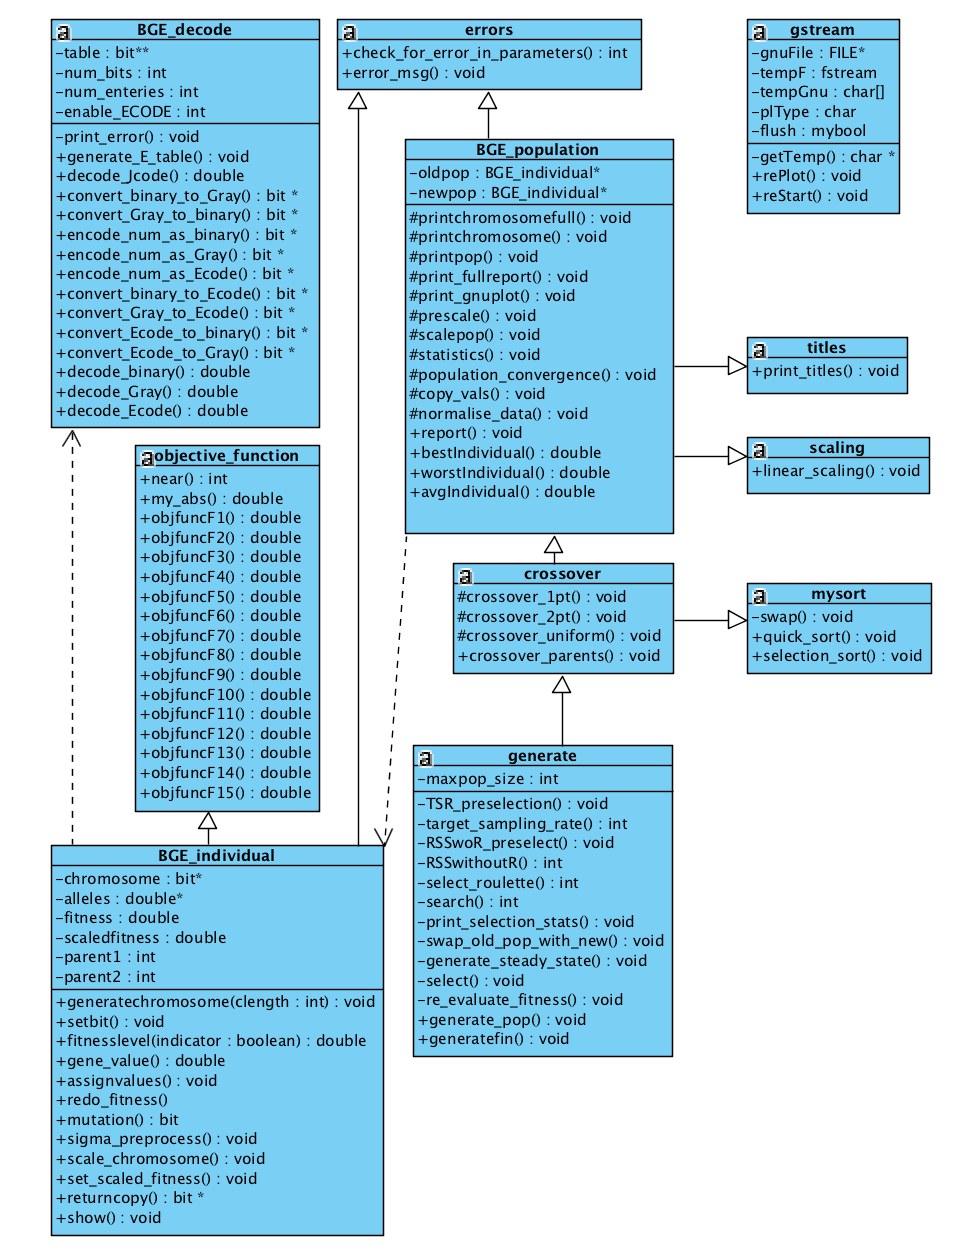
\includegraphics[width=1.3\linewidth]{figs/sga_class_diagram.png}
    }
    \caption{Class diagram of Object-oriented SGA}
     \label{fig:sga_classdiagram}
\end{figure}

\section{Issues with MPI support for Object-oriented paradigm}
The major drawback discovered with object-oriented implementation of GAs was the MPI's lack of support for object-oriented languages. The MPICH 3.2 version of MPI implementation were used this project. With further research on this topic it was discovered none of the major MPI implementation(OpenMPI, ) truly supported the object-oriented C++ other than just the compiler support.

In a conference article titled \textit{"Object Oriented MPI (OOMPI): a class library for the Message Passing Interface"} Squyres et al discussed MPI's lack of support of C++ class libraries and binding. In that paper they suggested an Object Oriented MPI specification \citep{squyresoompi}. However, this effort have been abandoned due to the lack of support from MPI community. After doing further research on this topic in Internet discussion forums and blog posts, it is found that there are ways of doing OO MPI using C++ by using third-party libraries Boost::mpi and Boost::serialization. Boost itself is a set of libraries for the C++ programming language that provide support for tasks and structures such as linear algebra, pseudorandom number generation, multithreading, image processing, regular expressions, and unit testing. Boost is a free to use library licensed under its own free, open-source license, known as the Boost Software License. An MPI program using the Boost::mpi library must initialise an mpi::environment object. This object initialises the MPI environment and enables communication among the processes. This object is initialised with the program arguments in the main program. The creation of this object initialises the MPI environment, and its destruction terminates it. The Boost::mpi requires objects to be serialised so that they are transmissible across processes. The Boost::serialization is a library for serialising C++ objects for sending/receiving data across network. To serialise a class one needs to define a template function serialize() in the class.

There is a little draw back with using Boost::mpi library. The Boost:mpi only implemented MPI1.1 which does not support many useful routines of MPI standards. Some people suggested to use that for regular programs. And for advanced programs to use mainstream MPI-3 libraries with Boost::Serialization for serialising C++ objects. Considering the scope of this project this options is not taken.
\section{Open Source Procedural GA}
A procedural implementation of GA based on Zbigniew Michalewicz's book \textit{"Genetic Algorithms + Data Structures = Evolution Programs"}\citep{michalewicz:96} available under GNU public license. The original version of this implementation was done by Dennis Cormier and Sita Raghavan. From Department of Scientific Computing at Florida State University John Burkardt made a C++ version of source code available on their department's website \citep{Burkardt:17}. The slightly refactored version of this source code without changing the actual algorithms is included in Appendix \ref{sourcecodes}. Where the original code is put into 4 separate source files shown in \ref{src:params.hpp}, \ref{src:sga_proc.hpp}, \ref{src:sga.cpp} \& \ref{src:sga_proc.cpp}.


This is a simple genetic algorithm implementation where the evaluation function takes positive values only and the fitness of an individual is the same as the value of the objective function.

Each generation involves selecting the best members, performing crossover and mutation and then evaluating the resulting population, until the terminating condition is satisfied.

Behaviour of this program is modified by defining parameters listed in Listing \ref{lst:procedural_ga_params} where POPSIZE is population size, MAXGEN is the number of generation to run, NVARS is the number of variables or genome in a chromosome, PXOVER and PMUTATION are the probabilities of crossover and  mutation respectively. However this program expects the permissible value ranges for each variable to be read from a text file.

\begin{lstlisting}[language=C, caption={Parameter definitions.}, label={lst:procedural_ga_params}]
# define POPSIZE 50
# define MAXGENS 1000
# define NVARS 3
# define PXOVER 0.8
# define PMUTATION 0.15
\end{lstlisting}

Listing \ref{lst:procedural_ga_struct} shows the data structure used for defining GENOTYPE which is a member of a population. The struct member .gene is a string of variables, .fitness is the fitness value .upper is the variable upper bounds, .lower: the variable lower bounds, .rfitness is the relative fitness and .cfitness is the cumulative fitness value. Relative and cumulative fitness values are used for elitist in a given generation.

\begin{lstlisting}[language=C, caption={GENOTYPE: Data structure of population member.}, label={lst:procedural_ga_struct}]
struct genotype
{
  double gene[NVARS];
  double fitness;
  double upper[NVARS];
  double lower[NVARS];
  double rfitness;
  double cfitness;
};
\end{lstlisting}

In Listing \ref{lst:procedural_ga_main} shows the for loop that is repeated for each generation cycle and perform the GA operations on current population. The select() procedure on line 3 perform a roulette wheel selection from current population. The elitist() procedure in line 9 performing an elitist operation which finds the best and the worst member of the current population. If the current best is better than last generation's best then replace it with current best otherwise replace the current worst with last generation best. 

\begin{lstlisting}[language=C, caption={Main loop controlling the GA operations.}, label={lst:procedural_ga_main}]
  for ( generation = 0; generation < MAXGENS; generation++ )
  {
    selector ( seed );
    crossover ( seed );
    mutate ( seed );
    report ( generation );
    evaluate ( );
    elitist ( );
  }
\end{lstlisting}


\subsubsection{Fitness function}
The fitness function provided with this code base is very simple one. This function was implemented to handle only three variables chromosome. It performs a very simple calculation of $ fitness = x_1^2 - x_1 * x_2 + x_3 $. As can be seen in source code provided in Appendix C, the original codebase is slightly modified to facilitate introducing other fitness function. The modification can be seen in Listing \ref{lst:pga_fitness}. 

\begin{lstlisting}[language=C, caption={Fitness function - Implementation of Griewank function}, label={lst:pga_fitness}]
void evaluate ( int my_start, int row_count )
{
    switch(FITNESS_F) {
        case F1:
            return f1(my_start, row_count);
            break;
        case F8:
            return f8(my_start, row_count);
            break;
        default:
            break;
    }
}
\end{lstlisting}

And for f8() the Griewank function was implemented as shown in Listing \ref{lst:proc_griewank}. The Griewank function is defined as below:

$fitness = 1 +  \sum_{i=1}^{i=n}(x_i^2/4000) - \prod_{i=1}^{i=n}cos(x_i/\sqrt{i}) $

\begin{lstlisting}[language=C, caption={Fitness function - Implementation of Griewank function}, label={lst:proc_griewank}]
void f8(int my_start, int row_count)
{
  int member;
  int i;
  double x[NVARS+1];
  double part1, part2;
  
  int ends = my_start + row_count;
  
  for ( member = my_start; member < ends; member++ )
  {
    for ( i = 0; i < NVARS; i++ )
    {
      x[i+1] = population[member].gene[i];
    }
    
    part1 = 0.0;
    for(i = 1; i < NVARS; i++)
    {
        part1 += pow(x[i], 2) / 4000;
    }
    
    part2 = 1.0;
    for(i = 1; i < NVARS; i++)
    {
        part2 *= cos( x[i] / sqrt(i) );
    }
       
    population[member].fitness = 1.0 + part1 - part2;
  }
  return;
}
\end{lstlisting}

\section{Parallelising Procedural GA using MPI}
\subsection{Parallel GA model}
The master-slave model of parallel GA is adopted for this implementation. The operation most commonly parallelised in master-slave model is the evaluation of the fitness function as in general this requires only individuals values not the entire population so that the communication is minimum between nodes. Parallelising the evaluation of fitness function is done by assigning a part of population to each node available in a cluster. Message passing occurs when slave nodes receive the subset of global population and returns evaluated fitness values to the master. 

Figure \ref{fig:flowchart_pga} represent the flowchart of implemented Parallel GA. Dotted line shows Message passing communication between Master and Slaves. This flowchart shows the diagram of implemented parallel GA using the procedural SGA discussed earlier in this section. As we can see from this diagram Master process responsible for initialising first generation of population, evaluate and report on them. The next task for the master process is to dividing up population among available slave processes. 

\begin{figure}[!hp]
    \vspace*{-1cm}
    \makebox[\linewidth]{
        \includegraphics[width=.9 \linewidth]{figs/flowchart_pga2.png}
    }
    \caption{Flowchart diagram of Implemented master-slave Parallel GA}
     \label{fig:flowchart_pga}
\end{figure}


The following subsections explain various MPI directives implemented.

\subsection{Initialising MPI environment}
As with all MPI program the message-passing environment needs to be initialised prior to calling any message-passing procedure. This is done by calling MPI\_Init() procedure on line 8 shown in the code fragments on Listing \ref{lst:pga_initialise_mpi}. MPI uses objects known as communicators and groups to define which collection of processes may communicate with each other. MPI\_Comm\_size() returns number of processes available for MPI communication and MPI\_Comm\_rank() returns its own unique rank id for identification within a communicator group.

\begin{lstlisting}[language=C, caption={Parallel GA implementation using MPI: Source code of main()}, label={lst:pga_initialise_mpi}]
MPI_Init(&argc, &argv);
MPI_Comm_size(MPI_COMM_WORLD, &numNodes); // How many nodes
MPI_Comm_rank(MPI_COMM_WORLD, &myId); // My Rank ID
\end{lstlisting}

\subsection{Creating MPI derived datatype for genotype}
MPI requires data to be in a contiguous memory location for marshalling and demarshalling of data to send and receive. Any non-primitive datatype needs to be defined for MPI to handle this properly. Listing \ref{lst:pga_mpi_create_struct} shows the procedure for creating a MPI derived datatype for the genotype struct of SGA. Line 14 contains the MPI routine MPI\_Type\_create\_struct() that requires 3 arrays containing information about user data types, their count and their offsets values within the struct along with original data type that is being converted and an MPI\_Datatype object where this routine will return the new type on success. In lines 7-12 the offsets values of genotype members are being stored in offsets array using C library macro offsetof() function.

\begin{lstlisting}[language=C, caption={Creating an MPI derived data type for genotype struct.}, label={lst:pga_mpi_create_struct}]
void create_mpi_genotype_struct(MPI_Datatype& mpi_genotype){
    const int nitems = 6;
    int blocklengths[6] = {NVARS, 1, NVARS, NVARS, 1, 1};
    MPI_Datatype types[6] = {MPI_DOUBLE, MPI_DOUBLE, MPI_DOUBLE, MPI_DOUBLE, MPI_DOUBLE, MPI_DOUBLE};
    
    MPI_Aint     offsets[6];
    offsets[0] = offsetof(genotype, gene);
    offsets[1] = offsetof(genotype, fitness);
    offsets[2] = offsetof(genotype, upper);
    offsets[3] = offsetof(genotype, lower);
    offsets[4] = offsetof(genotype, rfitness);
    offsets[5] = offsetof(genotype, cfitness);
    
    MPI_Type_create_struct(nitems, blocklengths, offsets, types, &mpi_genotype);
    MPI_Type_commit(&mpi_genotype);
}
\end{lstlisting}


\subsection{Partitioning of data}
Following strategy shown in Listing \ref{lst:pga_partitioning} is applied to partition the population among available nodes. A 2D array node\_data[][] shown in line 1 is used to hold the starting index and the row count for a given node id. From line 3 to line 11 the starting index and row counts are calculated and stored in node\_data[][] array for each node\_id. 

\begin{lstlisting}[language=C, caption={Partitioning population data among nodes}, label={lst:pga_partitioning}]
    int nodes_data[numNodes][2]; // Array to hold data partition information
    int start_i, num_rows;
    int chunk_size = (int)(ceil((double) POPSIZE / numNodes));
               
    for(int i = 0; i < numNodes; i++)
    {
        start_i = i * chunk_size;
        num_rows = min(chunk_size, POPSIZE - start_i);
        nodes_data[i][0] = start_i;
        nodes_data[i][1] = num_rows;
    }
\end{lstlisting}

\subsection{PGA v1}

\subsubsection{Master-Slave Communication}
In master-slave model all processes run the same MPI program. But depending on its role each process executes parts of the program. The parts of the main() shown in Listing \ref{lst:pga_mpi_main}. On line 3 each process gets its own communicator ID by calling MPI\_Comm\_rank(). Using this ID master process executes the master\_process() (line 5) and all other process executes slave\_process()(line 9). 

\begin{figure}[!htb]
        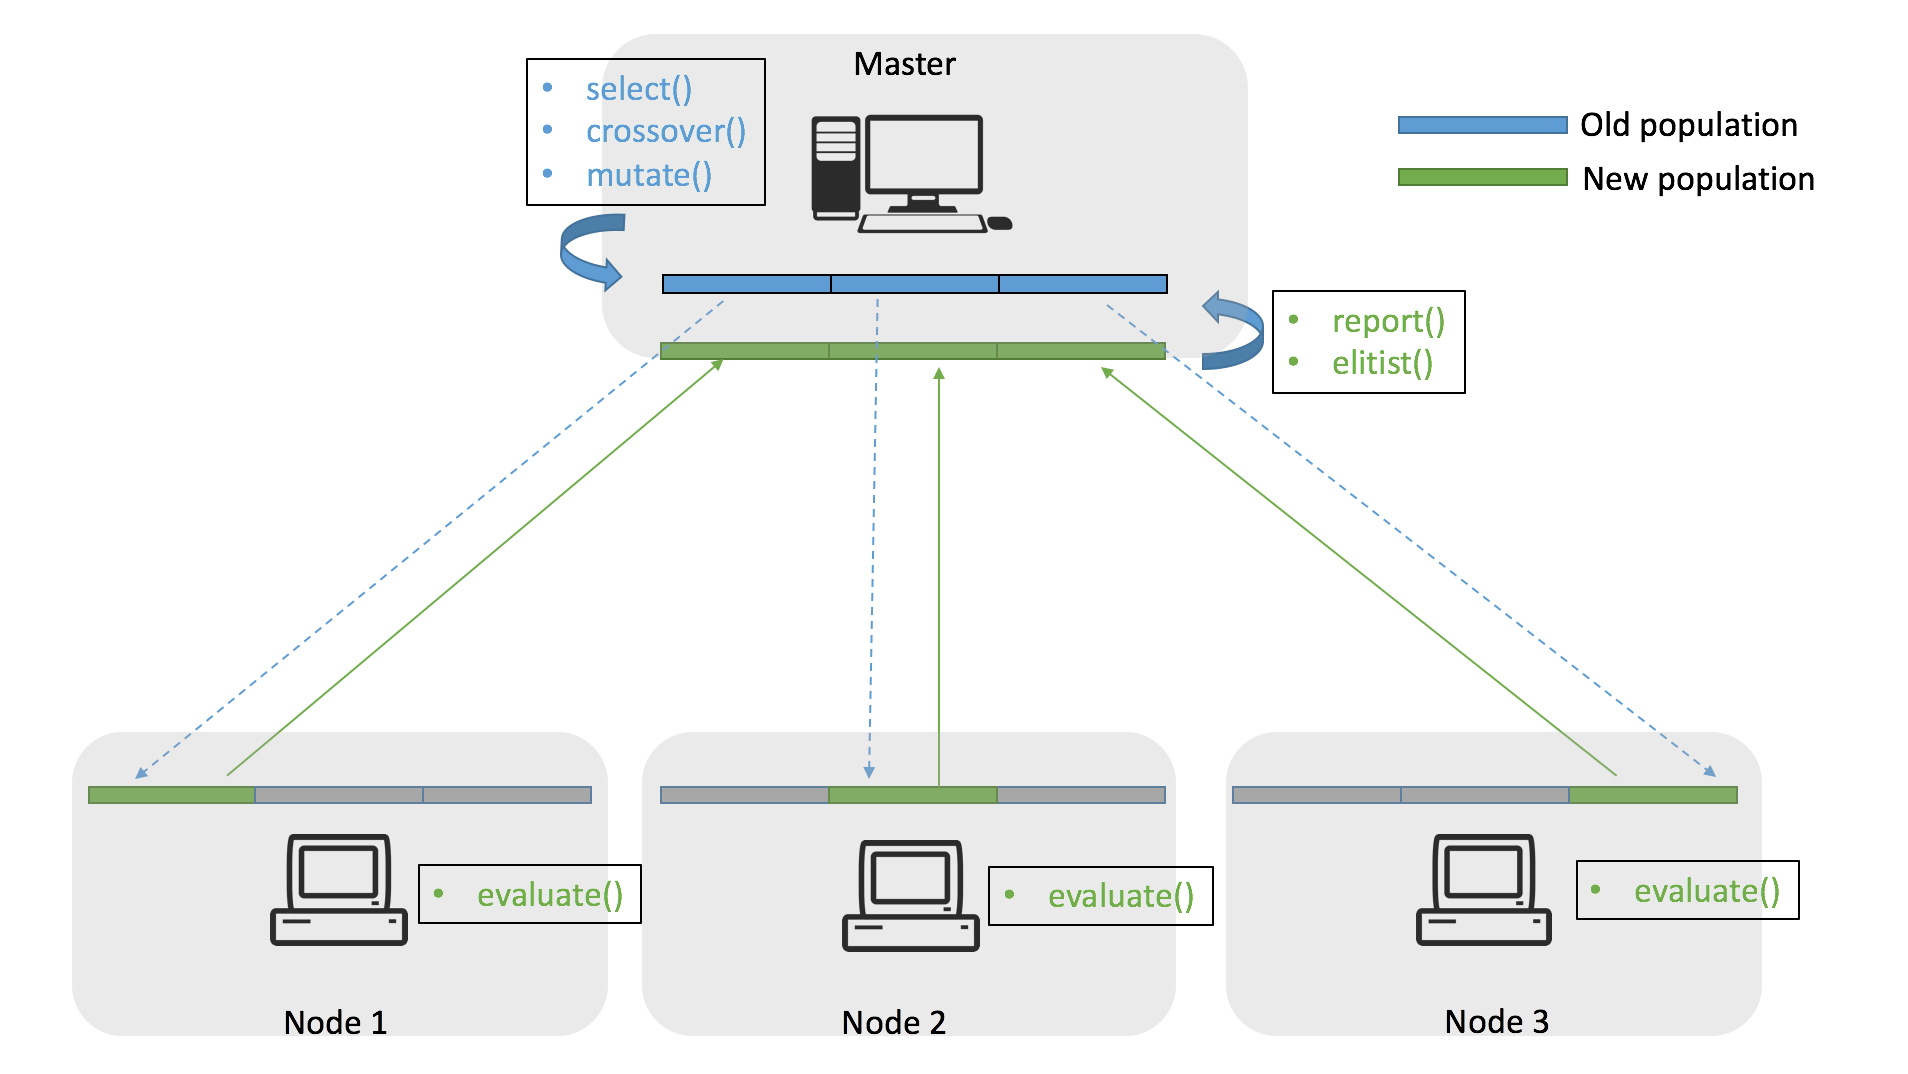
\includegraphics[width= \linewidth]{figs/pga_model_v1.png}
    \caption{PGA v1 model}
     \label{fig:pga_model_v1}
\end{figure}

For each generation, the master\_process() is responsible for performing selection, crossover and mutation operation on entire population ,  dividing population among all available nodes, updating all nodes with their parts of current population, collecting evaluated fitness values from each nodes, evaluate the best member for that generation, report and perform elitist operation on entire population. Where slave process is only responsible to receive a subset of population from master, evaluate their fitness values, send them back to master.  Figure \ref{fig:pga_model_v1} shows the master and slave data decomposition and the GA operation they perform on the population data depends on their role.

\begin{lstlisting}[language=C, caption={Master and slave pr}, label={lst:pga_mpi_main}]
ierr = MPI_Init(&argc, &argv);
ierr = MPI_Comm_size(MPI_COMM_WORLD, &numNodes); // How many nodes
ierr = MPI_Comm_rank(MPI_COMM_WORLD, &myId); // My Rank ID
    
if(myId == MASTER_ID) // Master Process
{
      master_process(filename, seed, mpi_genotype, nodes_data, start);
}
else // Slave processes
{  
    slave_process(seed, mpi_genotype, nodes_data);
}
\end{lstlisting}

\subsubsection{Master process}
In Listing \ref{lst:pga_master_process} parts of the master\_process() procedure is shown. After initialising the initial population master starts performing GA operation on them(lines 3-6). On lines 9-14 it starts sending subset of population to each nodes using MPI\_Send() routine. As we shall see in Listing \ref{lst:pga_slave_process} there is a corresponding MPI\_Recv routine call (line 2) invoked by the slave process. Master then evaluate it's own parts the population subset (line 17). On lines 20-25 master starts to gather the parts of population which have their fitness value calculated by the slave nodes. Then on line 27 master perform elitist() operation using entire population.

\begin{lstlisting}[language=C, caption={The master\_process() procedure.}, label={lst:pga_master_process}]
for(int generation = 0; generation < MAXGENS; generation++)
{   
      selector ( seed );
      crossover ( seed );
      mutate ( seed );     
      report(generation);

      int start_index, item_count;
      for(int nodeId = 1; nodeId < numNodes; nodeId++)
      {
          start_index = nodes_data[nodeId][0];
          item_count = nodes_data[nodeId][1];
          MPI_Send(&population[start_index], item_count, mpi_genotype, nodeId, SEND_DATA_TAG, MPI_COMM_WORLD);
        }
        
      /* Evaluate master's parts of the population */
      evaluate(nodes_data[0][0], nodes_data[0][1]);
        
      /* Collect all parts of new population from each node */
      for(int nodeId = 1; nodeId < numNodes; nodeId++)
      {
          start_index = nodes_data[nodeId][0];
          item_count = nodes_data[nodeId][1];
          MPI_Recv(&population[start_index], item_count, mpi_genotype, nodeId, RETN_DATA_TAG, MPI_COMM_WORLD, &status);
       }
                
      elitist();
}
\end{lstlisting}

\subsubsection{Slave process}
As we can see in Listing \ref{lst:pga_slave_process} the slave process starts with a MPI\_Recv() call on line 4. After receiving the parts for the population slave process perform evaluate() using its own starting index and row count on line 7. When the fitness evaluation is done it start to send the population part to master process by calling MPI\_Send() routine.


\begin{lstlisting}[language=C, caption={The slave\_process() procedure.}, label={lst:pga_slave_process}]
for(int generation = 0; generation < MAXGENS; generation++)
{
    /* Get a subset of population from master */
    ierr = MPI_Recv(&population[my_start], row_count, mpi_genotype, MASTER_ID, SEND_DATA_TAG, MPI_COMM_WORLD, &status);
        
    /* Perform fitness evaluation */
    evaluate (my_start, row_count);
        
    /* Send evaluated population to master */
    MPI_Send(&population[my_start], row_count, mpi_genotype, MASTER_ID, RETN_DATA_TAG, MPI_COMM_WORLD);
}
\end{lstlisting}


\subsection{PGA v2}
\subsubsection{Performance issue with PGA v1}
The first implementation of Master-slave GA as in PGA v1 distribute evaluation of fitness function among several slave processors while master executes the GA operations(selection, crossover and mutation). This implementation explore the search space in exactly same manner as a serial GA and follows exactly the same simple GA design guidelines. It is thought to be the case that, this implementation of master-slave parallel GA results in significant improvement in performance. However, as we shall see in Chapter \ref{empirical} when empirical studies were carried out the actual performance gains seemed to be worse than the serial GA. This is perhaps for the frequent MPI communication overhead that required in each generation for evaluating fitness values back and forth to the master and slave nodes. The execution time time of master-slave GAs have two components; the time used for communication between nodes and the time used in computation. So, the other reason is, master is responsible for performing all GA operations on entire population while slave nodes are mostly sitting idle during this time. With this approach slave nodes are under utilised where master node has a lot of workload 

So, in this version of PGA we tried to leverage some of the GA operations as well as evaluating fitness values to the slave nodes. The movements of population data and node specific GA operations are depicted in Figure \ref{fig:pga_model_v2}.

\begin{figure}[!htb]
        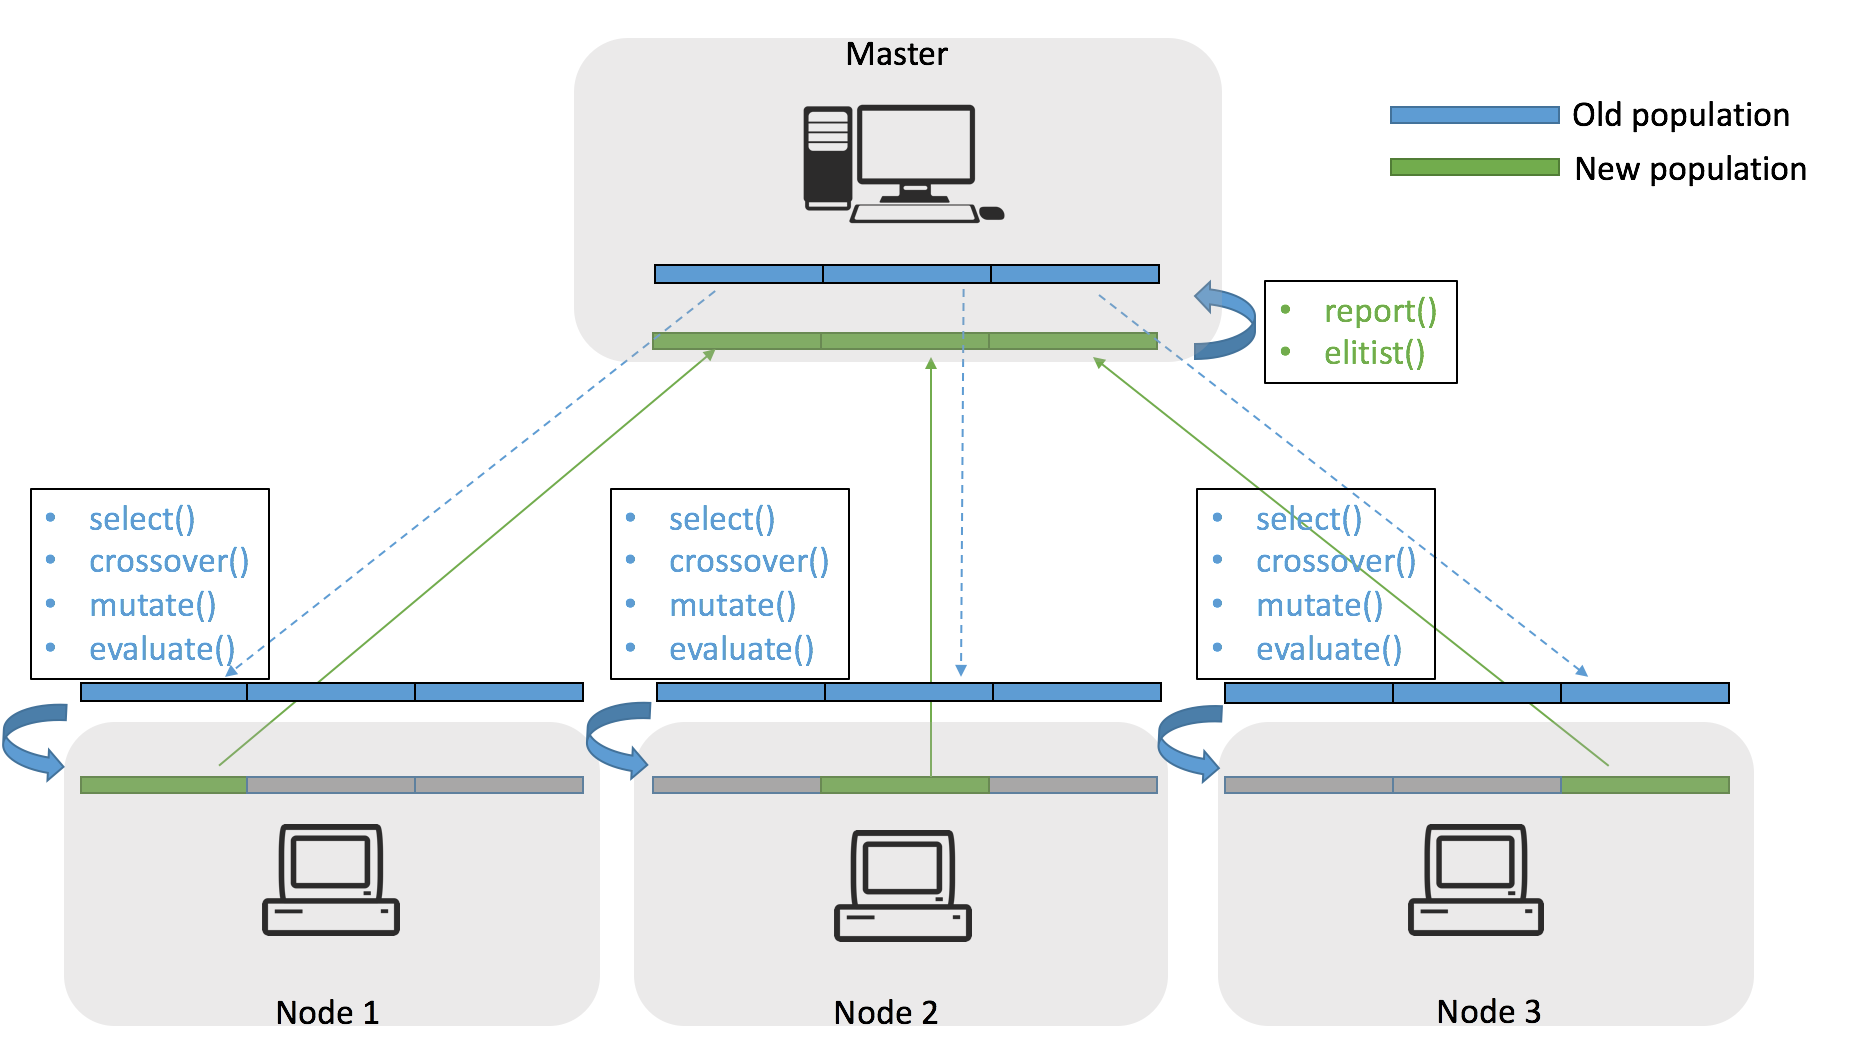
\includegraphics[width= \linewidth]{figs/pga_model_v2.png}
    \caption{PGA v2 model}
     \label{fig:pga_model_v2}
\end{figure}

\subsubsection{Using MPI Broadcast instead of explicit MPI Send/Recv}
To reduce communication overhead MPI collective routine \textbf{MPI\_Bcast()} is used by replacing  explicit \textbf{MPI\_Send() and MPI\_Recv()}. To ensure proper synchronisation among all nodes in the cluster the \textbf{MPI\_Barrier()} is called. When a process calls MPI\_Barrier(), it waits until all of the nodes also call this procedure.

Some part of this implementation is shown in Listing \ref{lst:pga_procedures}. On lines 5-9 master node initialises initial population and perform first elitist operation(keep\_the\_best( )). Slave nodes wait for these operation to complete because of MPI\_Barrier() call on line 12. On line 15 entire population is broadcasted with MPI\_Broadcast() call followed by another call to MPI\_Barrier().  On lines 20-21 all nodes determine their own data partition information. Then all nodes perform GA operations and evaluate the fitness values for the subpopulation(lines 22-27). On lines 32-36 each node then broadcasts its part of the population data. This followed by another synchronisation on line 38 before master node call the elitist() operation on entire population on line 43.

\begin{lstlisting}[language=C, caption={PGA v2 main() procedures.}, label={lst:pga_procedures}]
ierr = MPI_Comm_size(MPI_COMM_WORLD, &numNodes); // How many nodes
ierr = MPI_Comm_rank(MPI_COMM_WORLD, &myId); // My Rank ID
    
/* Initialise first gen population in master process */   
if(myId == MASTER_ID) // Master Process
{        
      initialize ( filename, seed );
      evaluate (0, POPSIZE );
      keep_the_best ( );
}

MPI_Barrier(MPI_COMM_WORLD);
   
/* Broadcast entire first generation from master process */
MPI_Bcast(population, POPSIZE + 1, mpi_genotype, MASTER_ID, MPI_COMM_WORLD);
   
MPI_Barrier(MPI_COMM_WORLD);
 
/* Each process does GA ops here on individual data parts */ 
int my_start = nodes_data[myId][0];
int row_count = nodes_data[myId][1];
for ( generation = 0; generation < MAXGENS; generation++ )
{      
     node_selector (my_start, row_count, seed );
     crossover ( seed );
     node_mutate ( my_start, row_count,seed );   
     evaluate (my_start, row_count);
         
       /* Sync message - 3 */
      MPI_Barrier(MPI_COMM_WORLD);
        
      for(int i = 0; i < numNodes; i++)
      {
          MPI_Bcast(&population[nodes_data[i][0]], nodes_data[i][1], mpi_genotype, i, MPI_COMM_WORLD);
          MPI_Barrier(MPI_COMM_WORLD);
      }
        
      MPI_Barrier(MPI_COMM_WORLD);
        
      if(myId == MASTER_ID) // Master Process
      {
          report(generation);
          elitist ( );
      }
        
      MPI_Barrier(MPI_COMM_WORLD);
}
\end{lstlisting}

\subsection{PGA v3}

\subsubsection{Running Time Analysis of node\_selector() Procedure}
\label{pga_runtime_analysis}
During empirical study of program running time, with PGA v2 we noticed some performance gain when number of processors are increased for smaller population size(5000). We also noticed there is a drop of speedup when population size is increased.

After a some investigation into this problem it was identified that the running time of \textbf{selector()} procedure is contributing for this unexpected result. The Listing \ref{lst:pga_select} parts of this procedure where we can see there is a nested for loop. The outer loop(line 2) on line has a range of \textit{$(0, n/p)$} and the inner loop(line 11) has a range of  \textit{$(0, p)$} where  \textit{n} is the population size and \textit{p} is number of processors. Thus this function has a running time complexity of $\mathcal{O}(n/p * n)$ which is essentially $\mathcal{O}(n^2)$.

Since, all nodes are executing this node\_selector() procedure using entire global population, the total running time is directly dependent upon the slowest node/processor in the cluster plus communication overheard for each generation cycles.


\begin{lstlisting}[language=C, caption={node\_select() procedure.}, label={lst:pga_select}]
/* Select survivors using cumulative fitness. */ 
for ( i = my_start; i < ends; i++ )
{ 
    p = r8_uniform_ab ( a, b, seed );
    if ( p < population[0].cfitness )
    {
        newpopulation[i] = population[0];   
    }
    else
    {
        for ( j = 0; j < POPSIZE; j++ )
        {
            if ( population[j].cfitness <= p && p < population[j+1].cfitness )
            {
                newpopulation[i] = population[j+1];
            }
        }
    }
}
\end{lstlisting}


\subsubsection{Limiting Selection to Partial Population}
Based on the analysis discussed above, in this implementation the \textbf{selector()} procedure is modified so that the selection is done using nodes local subpopulation. Thus this would result in running time complexity of $\mathcal{O}((n/p) * (n/p))$ i.e . $\mathcal{O}((n/p)^2)$ Theoretically, if we could add more nodes i.e. processors we could reduce the affect of population size increases for this procedure proportionally. We know that number of processor cannot always be matched with population size increases but for a reasonably large population size (not infinite), adding in extra nodes can reduce the running time complexity of this function significantly. Figure \ref{fig:pga_model_v3} shows the data partition and GA operation for master and slave nodes. All GA operation including selection is done on subpopulation.

\begin{figure}[!htb]
        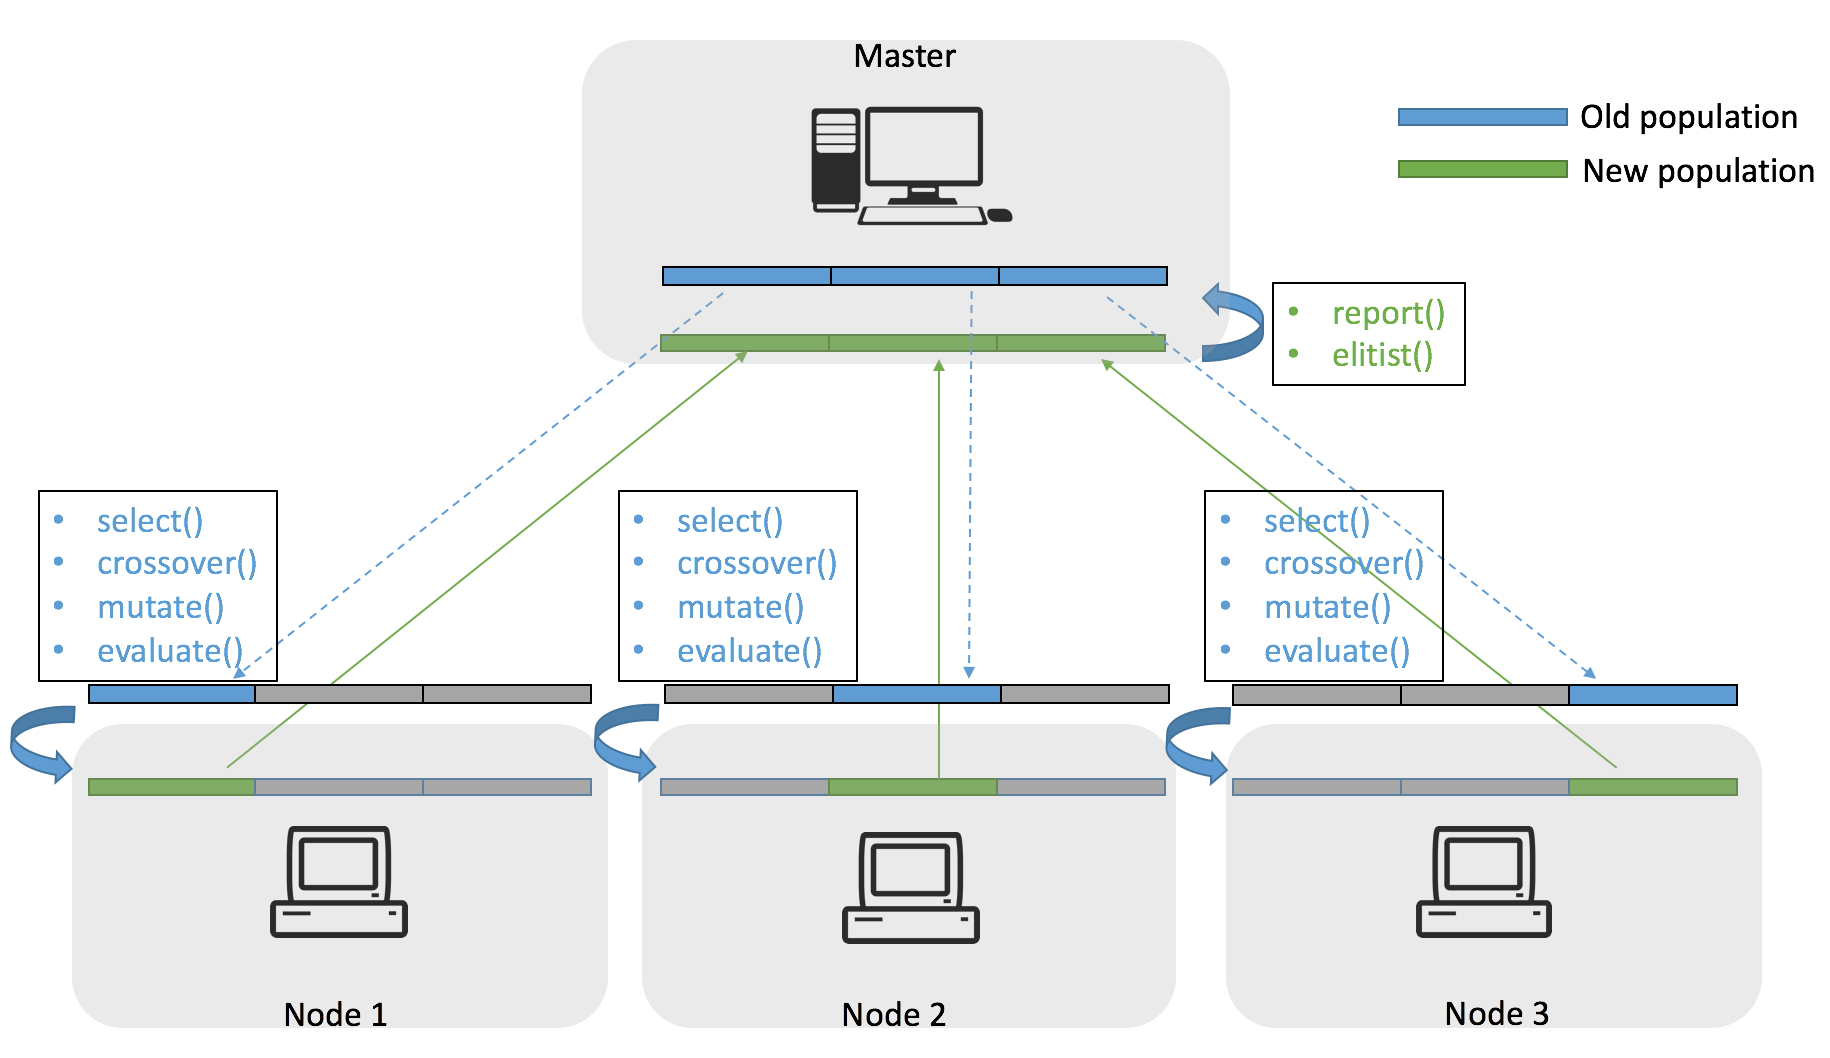
\includegraphics[width= \linewidth]{figs/pga_model_v3.png}
    \caption{PGA v3 model}
     \label{fig:pga_model_v3}
\end{figure}

Changes to the selector functions are shown in Listing \ref{lst:pga_select_changes} where the range inner for loop at line 10 is limited for the local subpopulation only which gives a range of \textit{$(0, n/p)$}.

\begin{lstlisting}[language=C, caption={Changes made in node\_select() procedures.}, label={lst:pga_select_changes}]
for ( i = my_start; i < ends; i++ )
{ 
    p = r8_uniform_ab ( a, b, seed );
    if ( p < population[my_start].cfitness )
    {
        newpopulation[i] = population[my_start];      
    }
    else
    {
        for ( j = my_start; j < ends; j++ )
        { 
            if ( population[j].cfitness <= p && p < population[j+1].cfitness )
            {
                newpopulation[i] = population[j+1];
            }
        }
    }
}
\end{lstlisting}

\subsection{Issues with Serialising Dynamic Data}
The SGA implementation allows population size, number of variables in a chromosome and number of generation can only be modified at compile time. To carry out the experiments we needed the PGA accept these parameters at runtime. So, an attempt was made to change these parameters at runtime with command line arguments. After a week of trials, this attempt was unsuccessful because of a number of reasons which are discussed here. Part of the problem was due to the data structure chosen to represent the chromosome which contains three static array members. The length of these arrays are defined at compile time. Population are initialised inside initialize\(\) procedure (Listing \ref{lst:initialize_proc}). Each individual is initialised with random permissible value. In this trial changes were made to the genotype data structure so that it could be initialised with dynamic arrays using malloc(). Program was compiled normally without any error. But during testing the PGA failed to produce acceptable outcome.

To find the underlying issue GDB was used to debug the problem. During this debugging program was run with a population size of 5. So the best member of a generation is kept  at index 5.
 
It was noticed(GDB output - Listing \ref{lst:gdb_output}) that some values of population members were changing unexpectedly. As we can see from the source code given in Appendix \ref{src:sga_proc.cpp} the initialize() procedure only assign initial value for \textbf{lbound}, \textbf{ubound} and \textbf{gene}. In this debugging session, the values of i, j and the best individual(population[5]) was monitored to catch unexpected any change. On line 42 we see that the value of  population[5].gene is 0x626330. But on next step on line 54 this value has changed to 0x3fe197d48c1f329c. We know that the initialize() procedure only assign values for the population member from 0 to (POPSIZE - 1) which is 4 in this run. So, the changes in population[5] is unexpected. It appeared that even though no value was assigned for best individual (which is population[5]), its member's values were changing. After looking more closely, it was noticed that the value that was being assigned to a data member for one individual was appearing inside some other individual's data member. Which means values were being assigned into wrong memory location. This indicated that malloc() for initialising the population array was not correct.


\begin{lstlisting}[style=BashInputStyle, label={lst:gdb_output}]
847 population[j].gene[i] = r8_uniform_ab ( lbound, ubound, seed );
1: population[5] = {fitness = 0, rfitness = 1.6304166312761136e-322, 
_ cfitness = 0, gene = 0x626330}
2: i = 0
3: j = 2
(gdb) 
840 for ( j = 0; j < POPSIZE; j++ )
1: population[5] = {fitness = 0, rfitness = 1.6304166312761136e-322, 
_ cfitness = 4.147546169663503, gene = 0x626330}
2: i = 0
3: j = 2
(gdb) 

.....

840 for ( j = 0; j < POPSIZE; j++ )
1: population[5] = {fitness = 0, rfitness = 1.6304166312761136e-322, 
_ cfitness = 4.147546169663503, gene = 0x626330}
2: i = 1
3: j = 1
(gdb) 
842 population[j].fitness = 0;
1: population[5] = {fitness = 0, rfitness = 1.6304166312761136e-322, 
_ cfitness = 4.147546169663503, gene = 0x626330}
2: i = 1
3: j = 2
(gdb) 
843 population[j].rfitness = 0;
1: population[5] = {fitness = 0, rfitness = 1.6304166312761136e-322, 
_ cfitness = 4.147546169663503, gene = 0x626330}
2: i = 1
3: j = 2
(gdb) 
844 population[j].cfitness = 0;
1: population[5] = {fitness = 0, rfitness = 1.6304166312761136e-322, 
_ cfitness = 4.147546169663503, gene = 0x626330}
2: i = 1
3: j = 2
(gdb) 
847 population[j].gene[i] = r8_uniform_ab ( lbound, ubound, seed );
1: population[5] = {fitness = 0, rfitness = 1.6304166312761136e-322, 
_ cfitness = 4.147546169663503, gene = 0x626330}
2: i = 1
3: j = 2
(gdb) 
840 for ( j = 0; j < POPSIZE; j++ )
1: population[5] = {fitness = 0, rfitness = 1.6304166312761136e-322, 
_ cfitness = 4.147546169663503, gene = 0x3fe197d48c1f329c}
2: i = 1
3: j = 2
(gdb) 
842 population[j].fitness = 0;
1: population[5] = {fitness = 0, rfitness = 1.6304166312761136e-322, 
_ cfitness = 4.147546169663503, gene = 0x3fe197d48c1f329c}
2: i = 1
3: j = 3
\end{lstlisting}

After this discovery, one and half week time was spent on how to allocate memory correctly for the \textbf{genotype} struct. But it seemed quite complicated to do so with three variable length array members in a struct. By researching on Internet about this, it was found that this issue is known as Variable Length Array In Struct(VLAIS). And with further research, some discussions related to this topic was found in Stackoverflow. The suggestions there were indicating that VLAIS is permissible on specific compiler i.e GCC C99 compatible only.  In one discussion posted on Stackoverflow \footnote{http://stackoverflow.com/questions/21804994/using-a-struct-member-as-array-size-in-the-same-struct} related to this topic further suggested that that variable-length arrays in structs is permissible in gcc (and the newest C-standards), but the variable array must always be the last member of the struct (so the compiler knows where all members are). In particular this means:

\begin{enumerate}
	\item There can be only one variable-length array
	\item If the struct is a member of another struct, it has to be the last member of that struct.
\end{enumerate}

Another post \footnote{http://stackoverflow.com/questions/17552312/multiple-flexible-array-in-a-struct-in-c} also suggested that it is not possible to have more than one flexible-array member in a struct.

There is no clear information whether mpic++ compiler has support for this feature of gcc too or not. The alternative solution to this problem would be to replace struct data structure with combination of C++ objects and vectors. Since this would have involved making a considerable changes to actual SGA implementation and possibilities of going back to the earlier problem with Object-oriented GA, a decision was made to leave these parameters to be defined at compile time.

\section{Testing}
To ensure the Parallel Genetic Algorithms implementations are producing expected outcome there is no alternative but to carry out testing. These tests were performed to validate the correctness of PGA implementation. We wanted to see if the output of the PGA program is consistent with the output of original SGA program using same parameters values and random seed.

\subsection{Test Configuration}
\label{test_config}
The common parameter values shown in Table \ref{tbl:test_params} are used for all testing both SGA and PGA programs.

\begin{table}[]
\centering
\caption{Parameters alues used with test cases.}
\label{tbl:test_params}
\begin{tabular}{|l|l|l|}
\hline
\textbf{Parameter}  & \textbf{Description }                        & \textbf{Value}     \\ \hline
POPSIZE    & Population Size                     & 5000      \\ \hline
MAXGENS    & Number of Generation                & 100       \\ \hline
NVARS      & Number of variables in a Chromosome & 3         \\ \hline
PXOVER     & Probability of Crossover            & 0.8       \\ \hline
PMUTATION  & Probability of Mutation             & 0.15      \\ \hline
FITNESS\_F & Fitness function (F8: Griewank)                   & F8        \\ \hline
SEED       & Random value generator seed         & 123456789 \\ \hline
Genome Encoding       & Encoding scheme for genome representaion         & Real value Encoding \\ \hline
\end{tabular}
\end{table}

As the original SGA was implemented with Real-value encoding scheme for genome representation the range of these values are given using a input file. For this test configuration with 3 genome per chromosome the permissible values are given as listed in Table \ref{tbl:genome_range}.

\begin{table}[]
\centering
\caption{Genome value range for 3 variables Griewank function}
\label{tbl:genome_range}
\begin{tabular}{|l|l|}
\hline
\textbf{Lower} & \textbf{Upper} \\ \hline
-512.0           & 511.0            \\ \hline
-512.0           & 511.0            \\ \hline
-512.0           & 511.0            \\ \hline
\end{tabular}
\end{table}

As discussed in section \ref{beowulf:process_manager} the hosts information entries shown in Listing \ref{lst:config_hydra} were added for Hydra (MPI Process Manager). The entry at line 1 is master node's hostname. Which means master node also is acting as a compute node in the cluster.

\begin{lstlisting}[style=BashInputStyle, label={lst:config_hydra}, caption={The hosts file configuration for Hydra.}]
padma:2
meghna:2
jamuna:2
\end{lstlisting} 

The PGA program was run by using following command:
\begin{lstlisting}[style=BashInputStyle, label={lst:run_mpi}]
$mpiexec -f ~/hosts -n 6 ./pga
\end{lstlisting}
The command \textbf{mpiexec} takes in parameter \textbf{-f} for the hosts file name and \textbf{-n} for  the number of processes that needs to be created in the cluster. The example shown above will launch 6 process that will run the executable binary \textbf{pga}.

\textbf{All tests results shown in this section are carried out in Hardware based Beowulf} system not in simulated cluster.

\subsection{Tests Outcome}
The GA programs output for the SGA, PGA v1, PGA v2 and PGA v3 are shown below. As these tests were run with a generation size if 100 the full output is not shown to save space. Instead, outputs are shown into two split images "Top part" and "Bottom part" of the screen capture that convey most important information. We are assuming the original SGA program is producing a correct output. Then the subsequent 3 PGA programs outputs are compared against SGA's output to validate and analyse each PGA implementation. 

\subsubsection{SGA Output}

Figures \ref{fig:test_sga_top} and \ref{fig:test_sga_bottom} shows the output of original SGA program compiled with the parameter configuration discussed in section \ref{test_config}.

\begin{figure}[!htb]
	\center
        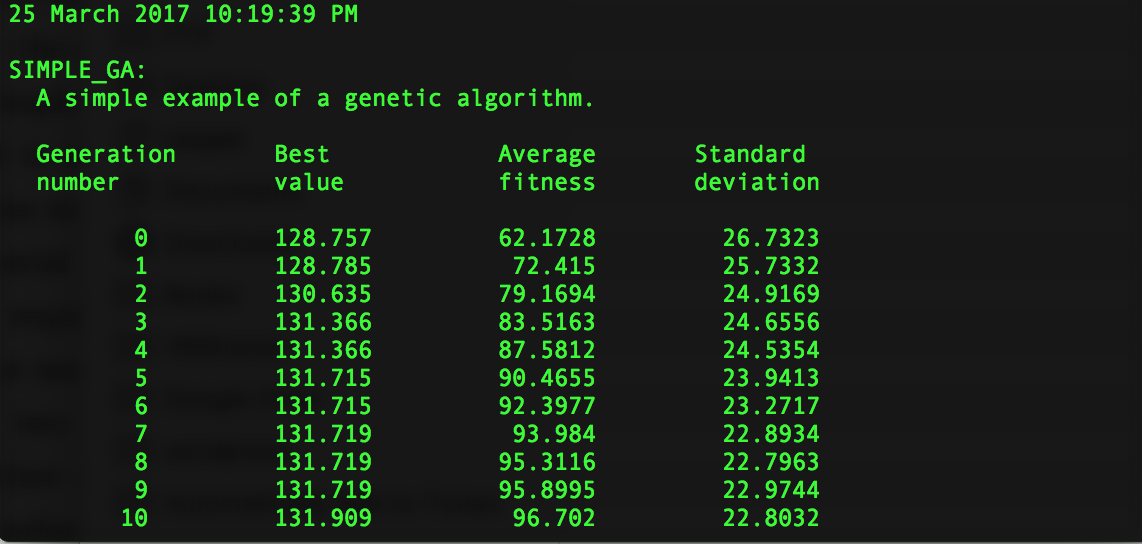
\includegraphics[width= \linewidth]{figs/tests/sga_top.png}
    \caption{SGA output - Top part}
     \label{fig:test_sga_top}
\end{figure}

\begin{figure}[!htb]
	\center
        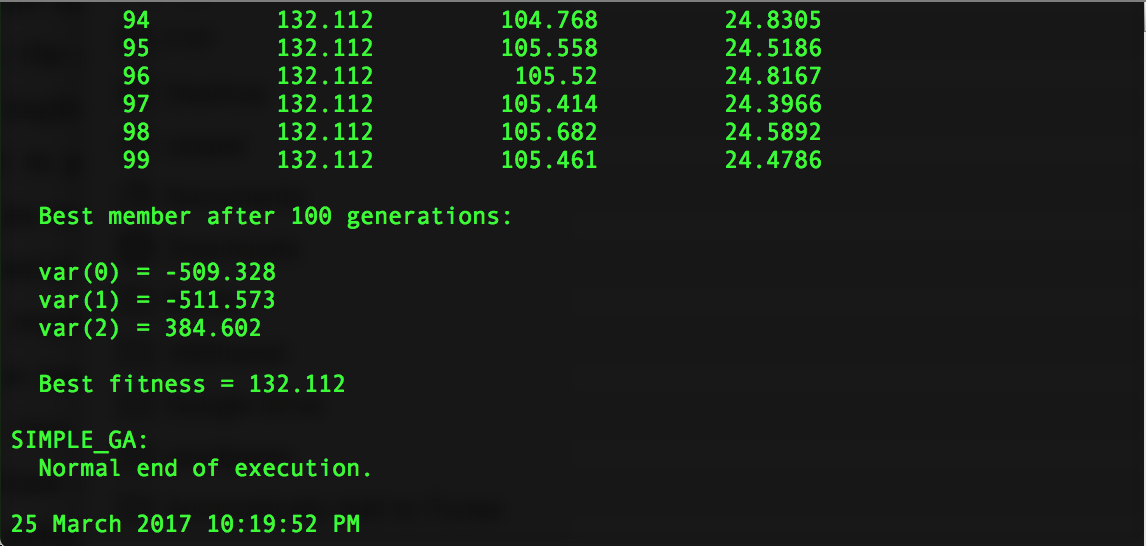
\includegraphics[width= \linewidth]{figs/tests/sga_bottom.png}
    \caption{SGA output - Bottom part}
     \label{fig:test_sga_bottom}
\end{figure}

\subsubsection{PGA v1 Output}

Figures \ref{fig:test_pga_top} and \ref{fig:test_pga_bottom} shows the output of original PGA v1 compiled with the parameter configuration discussed in section \ref{test_config}.

\begin{figure}[!htb]
	\center
        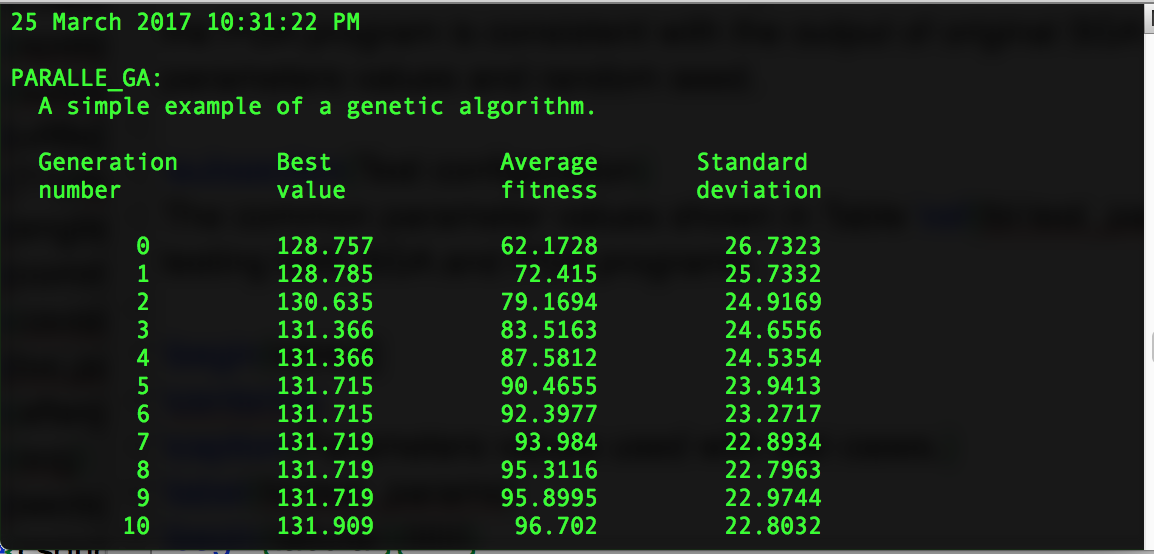
\includegraphics[width= \linewidth]{figs/tests/pga_top.png}
    \caption{PGA v1 output - Top part}
     \label{fig:test_pga_top}
\end{figure}

\begin{figure}[!htb]
	\center
        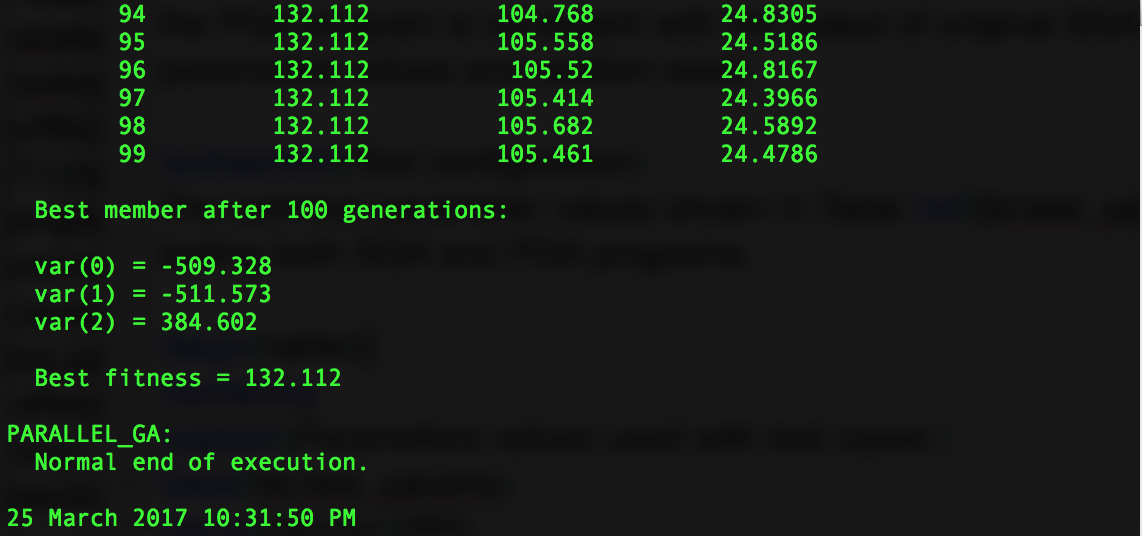
\includegraphics[width= \linewidth]{figs/tests/pga_bottom.png}
    \caption{PGA v2 output - Bottom part}
     \label{fig:test_pga_bottom}
\end{figure}

\subsubsection{PGA v2 Output}

Figures \ref{fig:test_pgav2_top} and \ref{fig:test_pgav2_bottom} shows the output of original PGA v2 compiled with the parameter configuration discussed in section \ref{test_config}.

\begin{figure}[!htb]
	\center
        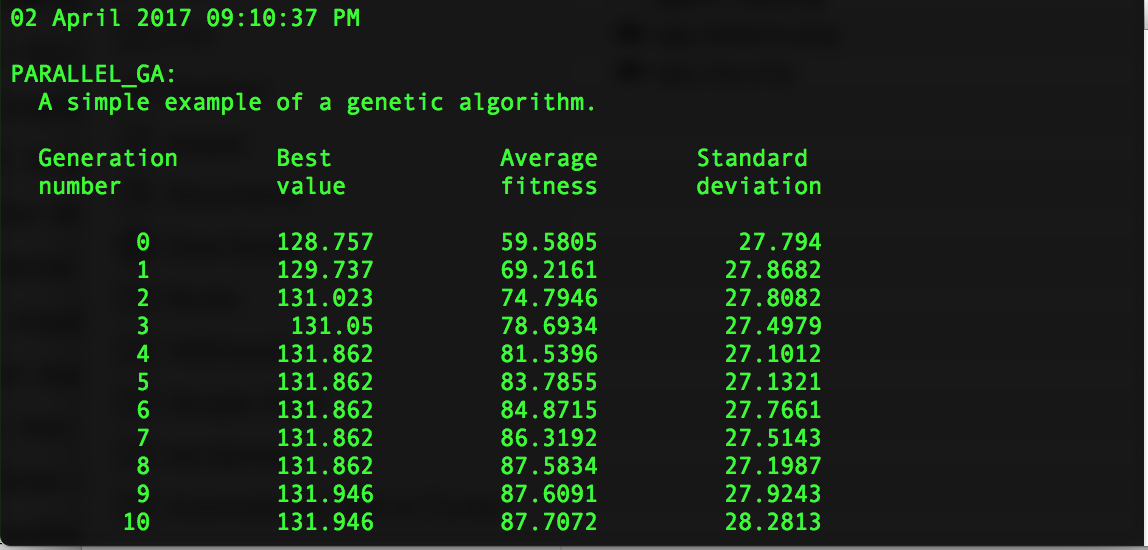
\includegraphics[width= \linewidth]{figs/tests/pgav2_top.png}
    \caption{PGA v1 output - Top part}
     \label{fig:test_pgav2_top}
\end{figure}

\begin{figure}[!htb]
	\center
        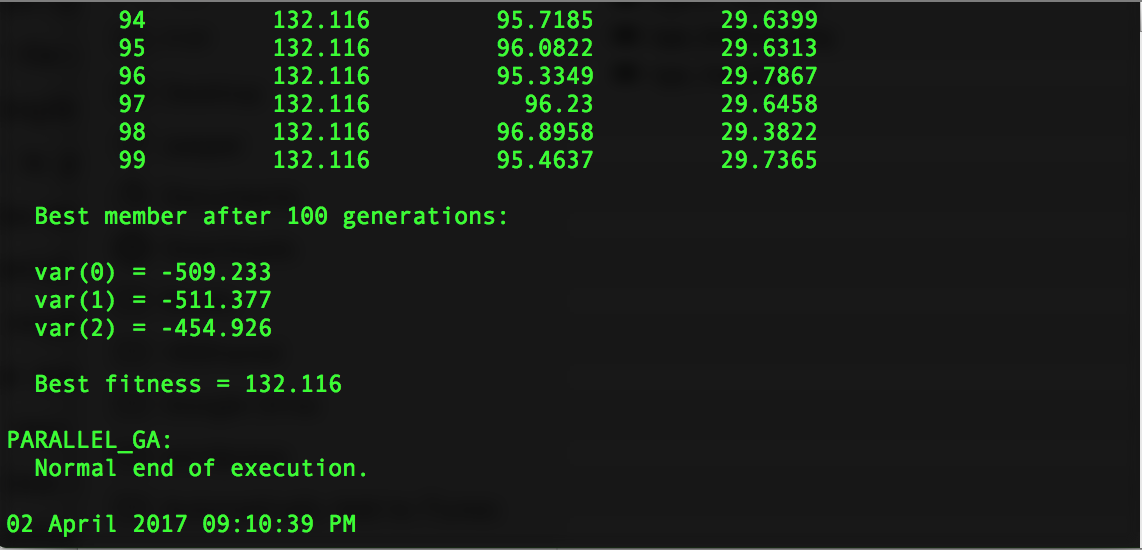
\includegraphics[width= \linewidth]{figs/tests/pgav2_bottom.png}
    \caption{PGA v2 output - Bottom part}
     \label{fig:test_pgav2_bottom}
\end{figure}

\subsubsection{PGA v3 Output}

Figures \ref{fig:test_pgav3_top} and \ref{fig:test_pgav3_bottom} shows the output of original PGA v3 compiled with the parameter configuration discussed in section \ref{test_config}.

\begin{figure}[!htb]
	\center
        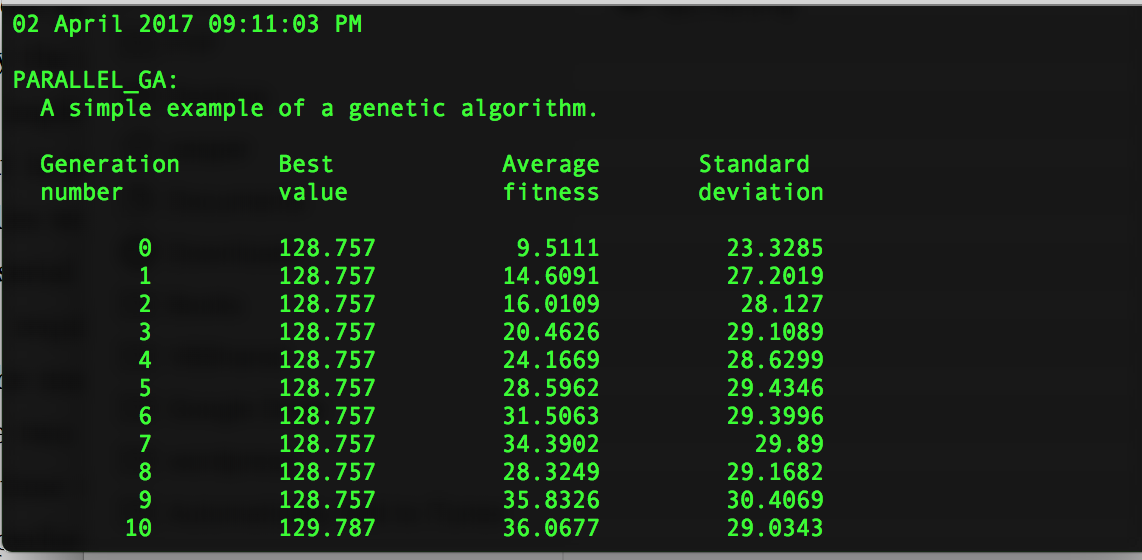
\includegraphics[width= \linewidth]{figs/tests/pgav3_top.png}
    \caption{PGA v3 output - Top part}
     \label{fig:test_pgav3_top}
\end{figure}

\begin{figure}[!htb]
	\center
        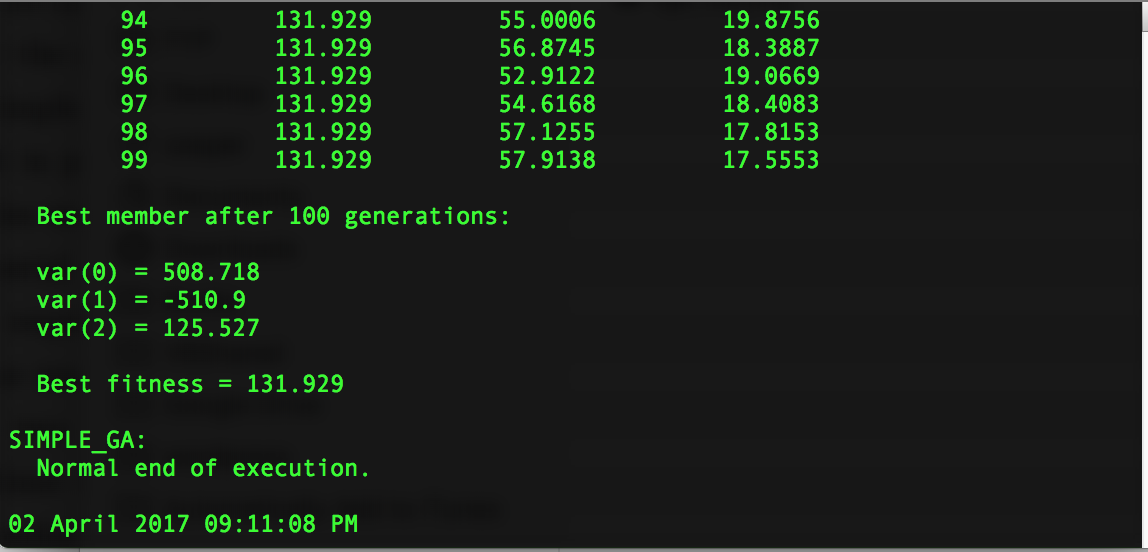
\includegraphics[width= \linewidth]{figs/tests/pgav3_bottom.png}
    \caption{PGA v3 output - Bottom part}
     \label{fig:test_pgav3_bottom}
\end{figure}

 



\section{Discussion}
The Beowulf implementation required a further steps for administrative tasks such and allowing remote access using vncserver, configuring ddns so that the system is accessible while not working from home. Since, the development needed the cluster setup to compile and and run MPI program the Integrated Development Environment set was also configured so that it able to use the remote cluster infrastructure. The necessary details are omitted here because of space constraint and they are not the main focus point of this project.

As described in previous section in this chapter, in this project we only explored one model of parallel GA which is master-slave model. In conjunction with the tests results and experiments shown in next chapter we see that pure master-slave model of PGA(PGA v1) did not give us any speed up at all, which is understandable since the communication overhead for message-passing actually more costly than actual computation done by multiple nodes. With PGA v2 where we changed the algorithm to utilise all nodes to do the GA operations instead of just computing fitness value we started to see speedup improvements. But this gains were not as much as expected. Lastly, in PGA v3 we limited the selection space to the subpopulation that a node operates on. This implementation gives us a good speedup gains. However, as we can see from the tests result of PGA v3 the actual outcome of GA is slightly worse than that of original SGA. That is because PGA v3 is close to a distributed PGA model as discussed in Section 2.5.3 without any migration policy. Next logical step of this project would be to implement a distributed model of PGA with a migration policy. Due to the time constraint of this project we needed to stop at the PGA v3.
